% Exact weighted graphs for K_tau + a K_(2 tau).
% C_t=(1-t)H_0+tH_1. Vertex numbers are Fourier indices, not eigenvalues.
% Requires only tikz and the manuscript's standard mathematical packages.
\begin{figure}[tbp]
\centering
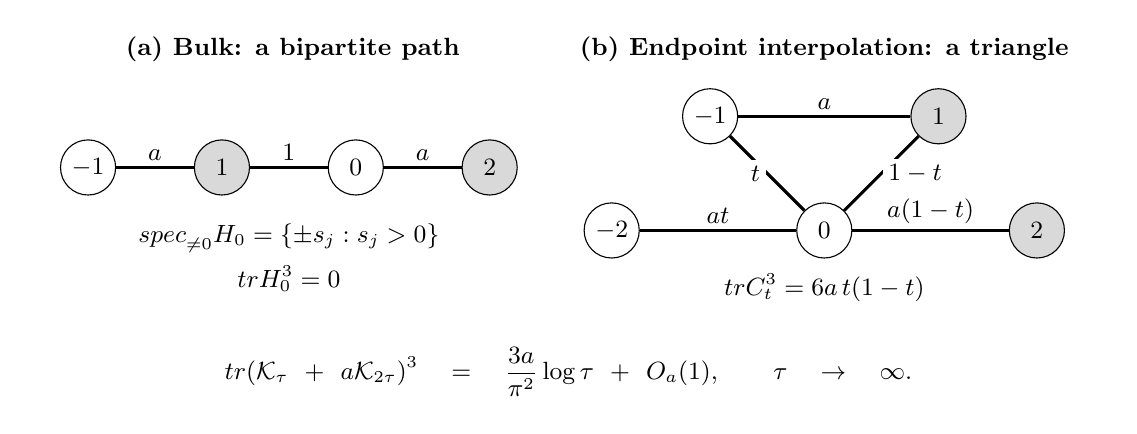
\begin{tikzpicture}[x=1cm,y=1cm,font=\small,
  vertex/.style={circle,draw,fill=white,minimum size=7mm,inner sep=0pt},
  positive/.style={vertex,fill=black!15},
  weight/.style={fill=white,inner sep=2pt}]
  \node[font=\small\bfseries] at (-3.50,1.50)
    {(a) Bulk: a bipartite path};
  \node[vertex] (bm) at (-6.10,0) {$-1$};
  \node[positive] (bp) at (-4.40,0) {$1$};
  \node[vertex] (bz) at (-2.70,0) {$0$};
  \node[positive] (bq) at (-1.00,0) {$2$};
  \draw[thick] (bm) -- node[weight,above] {$a$} (bp);
  \draw[thick] (bp) -- node[weight,above] {$1$} (bz);
  \draw[thick] (bz) -- node[weight,above] {$a$} (bq);
  \node[align=center] at (-3.55,-1.15)
    {$\operatorname{spec}_{\ne0}H_0=\{\pm s_j:s_j>0\}$\\[4pt]
     $\operatorname{tr}H_0^3=0$};
  \node[font=\small\bfseries] at (3.25,1.50)
    {(b) Endpoint interpolation: a triangle};
  \node[vertex] (cm) at (1.80,0.65) {$-1$};
  \node[positive] (cp) at (4.70,0.65) {$1$};
  \node[vertex] (cz) at (3.25,-0.80) {$0$};
  \node[vertex] (cl) at (0.55,-0.80) {$-2$};
  \node[positive] (cr) at (5.95,-0.80) {$2$};
  \draw[line width=1.1pt] (cm) -- node[weight,above] {$a$} (cp);
  \draw[line width=1.1pt] (cm) -- node[weight,left] {$t$} (cz);
  \draw[line width=1.1pt] (cp) -- node[weight,right] {$1-t$} (cz);
  \draw[thick] (cl) -- node[weight,above] {$at$} (cz);
  \draw[thick] (cz) -- node[weight,above] {$a(1-t)$} (cr);
  \node at (3.25,-1.53) {$\operatorname{tr}C_t^3=6a\,t(1-t)$};
  \node[align=center,text width=13.5cm] at (0,-2.60) {
    $\displaystyle
    \operatorname{tr}(\mathcal K_\tau+a\mathcal K_{2\tau})^3
       =\frac{3a}{\pi^2}\log\tau+O_a(1),\qquad \tau\to\infty.$};
\end{tikzpicture}
\caption{Exact weighted graphs for the two-harmonic family.
Vertices are Fourier indices; shaded vertices have positive index.
Isolated zero vertices are omitted in (a).
Every bulk edge joins the two index classes, so the bulk spectrum is
sign-symmetric. For $C_t=(1-t)H_0+tH_1$, the three edges on
$\{-1,0,1\}$ have product $a\,t(1-t)$.
The six oriented closed walks around this triangle give the cubic trace.
The logarithmic law also uses the polynomial localization and scalar
sawtooth calculation proved in the text. Here $a\in\mathbb R$ is fixed;
the triangle is present when $a\ne0$ and $0<t<1$.}
\label{fig:unified-two-harmonic}
\end{figure}
